\documentclass[11pt]{article}
\usepackage[margin=1in]{geometry}
\usepackage{amsmath,amssymb,amsthm,mathtools}
\usepackage{booktabs}
\usepackage{enumitem}
\usepackage{float}
\usepackage{graphicx}
\usepackage[colorlinks=true,citecolor=blue,linkcolor=blue,urlcolor=blue]{hyperref}
\usepackage[capitalize,nameinlink]{cleveref}
\usepackage[numbers,sort&compress]{natbib}

\newtheorem{theorem}{Theorem}[section]
\newtheorem{proposition}[theorem]{Proposition}
\newtheorem{lemma}[theorem]{Lemma}
\newtheorem{corollary}[theorem]{Corollary}
\theoremstyle{definition}
\newtheorem{condition}[theorem]{Condition}
\theoremstyle{remark}
\newtheorem{remark}[theorem]{Remark}

\newcommand{\C}{\mathbb C}
\newcommand{\Id}{\mathrm I}
\newcommand{\HS}{\mathfrak S_2}
\newcommand{\cE}{\mathcal E}
\newcommand{\cF}{\mathcal F}
\newcommand{\cI}{\mathcal I}
\newcommand{\cL}{\mathcal L}
\newcommand{\cQ}{\mathcal Q}
\newcommand{\spr}{\operatorname{spr}}
\newcommand{\tr}{\operatorname{tr}}
\newcommand{\Ran}{\operatorname{Ran}}
\newcommand{\norm}[1]{\left\lVert #1\right\rVert}

\title{Factor-Aware Sparse-to-Full Transfer for Intrinsic Riesz Identification\\
\large Growing-Horizon Hardy Robustness, a Conditional Closure Theorem,
and a Nonnormal No-Go}
\author{Liang Wang}
\date{July 2026}

\begin{document}
\maketitle

\begin{abstract}
The small-noise intrinsic-identification program for a folded-Gaussian
quadratic transfer operator has reduced the continuum defect to two
directional Hardy energies.  Previous work supplied deterministic
finite-matrix tail certificates and an adaptive sparse approximation, but
did not propagate the cutoff through the matrix's own Riesz factors and
normalized Haar coupling ranges.  We close that finite-dimensional
interface.

First, a Hilbert--Schmidt coupling perturbation
$\norm{B-\widetilde B}_{\HS}\le\varepsilon_B<\norm B_{\HS}$ gives
\[
 \left\|
 \frac B{\norm B_{\HS}}-
 \frac{\widetilde B}{\norm{\widetilde B}_{\HS}}
 \right\|_{\HS}
 \le\frac{2\varepsilon_B}{\norm B_{\HS}}.
\]
Since adjacent folded-Gaussian couplings have size
$\Theta(h\sigma^{-3/2})$, an adaptive cutoff error of order
\[
 \frac{h^2}{(\log(1/h))^{1/4}}
\]
is automatically negligible after normalization.  Second, we give explicit
left/right defect formulas for the
intrinsic triples in terms of the Markov, unweighted-projector,
weighted-Riesz, and coupling defects.  Third, actual finite-time ledgers
$a_j=\norm{A^j}$ and $\widetilde a_j=\norm{\widetilde A^j}$ yield
\[
 d_M=\delta_A\sum_{j=0}^{M-1}a_{M-1-j}\widetilde a_j,
 \qquad q_M+d_M<1,
\]
which transports a growing-horizon block contraction and a complete Hardy
upper without replacing nonnormal transients by powers of $\norm A$.

The resulting synthesis is exact but conditional: if the dyadic left and
right Hardy budgets are $O(\sigma^{-\alpha_B})$ and
$O(\sigma^{-\alpha_C})$, with range-restricted residues bounded, then
\[
 \norm{\cI_{n,\sigma}}_{\HS}
 =O\!\left(n^{-2}\sigma^{-13/4-\alpha_B-\alpha_C}\right).
\]
Every strict $n\sigma^2\to\infty$ schedule survives when
$\alpha_B+\alpha_C\le1/4$; polylogarithmic budgets give the expected
$n^{-2}\sigma^{-13/4}\operatorname{polylog}(1/\sigma)$ law.  We also prove
that small matrix error alone cannot control nonnormal Riesz factors, so a
contour-conditioning or strong--weak stability ledger is indispensable.
A five-scale dense audit through dimension $512$ and a 256-bit Arb
arithmetic audit confirm the transfer mechanism, but do not prove the
remaining dyadically uniform Hardy or Riesz-conditioning premises.
\end{abstract}

\noindent\textbf{Keywords:} Riesz projection; nonnormal perturbation;
Hilbert--Schmidt Hardy energy; growing horizon; Gaussian cutoff; intrinsic
Galerkin identification.

\noindent\textbf{MSC 2020:} 47A10; 47B10; 65F35; 65G20; 93B36.

\section{Introduction}

For each positive noise width $\sigma$, the folded-Gaussian quadratic
operator has two simple peripheral branches: the Perron root and a negative
parity resonance approaching $-1$.  Subtracting their intrinsic weighted
Riesz terms produces the bulk relevant to the two-step trace and determinant
program.  The continuum terms themselves are spatially resolved under the
strict mesh condition $n\sigma^2\to\infty$, but a finite Galerkin matrix
recomputes its own spectral terms.  The remaining defect is therefore
\[
 \cI_{n,\sigma}
 =\cQ_{\rm per}(E_n\mathcal K_\sigma E_n)
  -E_n\cQ_{\rm per}(\mathcal K_\sigma)E_n.
\]

RH-48 expressed this defect as an exact dyadic sum and proved that a mixed
directional gain $O(\sigma^{-\gamma})$ gives
\begin{equation}
 \norm{\cI_{n,\sigma}}_{\HS}
 =O(n^{-2}\sigma^{-3-\gamma}).
 \label{eq:rh48}
\end{equation}
The strict bulk-square mesh range survives for $\gamma\le1/2$
\citep{WangIntrinsic2026}.  RH-49 replaced the mixed gain by a purely
Hilbert--Schmidt gain $\cF_{n,\sigma}$ at a sharp quarter-power stable-rank
cost.  Thus $\cF=O(\sigma^{-\delta})$ gives
\begin{equation}
 \norm{\cI_{n,\sigma}}_{\HS}
 =O(n^{-2}\sigma^{-13/4-\delta}),
 \qquad \delta\le\frac14
 \label{eq:rh49}
\end{equation}
as the full-range threshold \citep{WangDirectional2026}.

RH-50 converted the two normalized reduced-resolvent actions into left and
right Hardy energies after exact Perron/parity removal
\citep{WangHardy2026}.  RH-52 proved that the explicit range-restricted
residues are $O(1)$ from weak intrinsic factors and established
\begin{equation}
 \norm B_{\HS},\norm C_{\HS}
 =\Theta(h\sigma^{-3/2})
 \label{eq:coupling-scale}
\end{equation}
along the cell-average schedules \citep{WangFactorTransfer2026}.  RH-51 and
RH-53 then replaced fixed-step contraction and a fitted time tail by
growing-horizon, deterministic all-column certificates
\citep{WangStructuredStein2026,WangHardyTail2026}.  The last uncomposed
finite-matrix interface was that a sparse/full Gaussian perturbation changes
the Riesz terms and the normalized coupling sources themselves.

This paper gives that composition.  Its role is deliberately narrower than
an unconditional Stage-A4 theorem.  The exact algebra determines which
Riesz-conditioning and Hardy-budget premises suffice, how their exponents
combine, and how a finite certificate transfers.  It does not derive the
remaining uniform premises from five computed noise levels.

\subsection*{Main results}

\begin{enumerate}[leftmargin=2.2em]
 \item Normalizing a nonzero Hilbert--Schmidt coupling costs at most twice
 its relative perturbation.  In combination with
 \eqref{eq:coupling-scale}, the adaptive Gaussian cutoff is harmless on the
 normalized coupling ranges.

 \item Common isolating contours give separate perturbation ledgers for the
 unweighted projectors and weighted Riesz terms.  These feed directly into
 the two intrinsic Hardy triples.

 \item The exact power telescoping identity, evaluated with actual
 finite-time norm ledgers, transfers a contracting block and gives a
 complete perturbed Hardy-energy upper.

 \item The RH-48--RH-53 chain composes with the exact exponent
 $\delta=\alpha_B+\alpha_C$.  The quarter-power threshold is therefore a
 budget shared by the two Hardy directions, not a quarter power available
 independently to each.

 \item A two-dimensional nonnormal family has matrix perturbation tending
 to zero while its peripheral Riesz projector changes by order one.  Thus
 cutoff convergence alone cannot close the intrinsic-factor interface.
\end{enumerate}

\section{Intrinsic directional triples}

Let $T$ be a fine matrix and let $U$ and $W$ be the coarse and Haar-detail
isometries.  Relative to the adjacent split,
\[
 T=\begin{pmatrix}T_c&B\\ C&D\end{pmatrix},
 \qquad B=U^*TW,
 \qquad C=W^*TU.
\]
For the two peripheral branches, write
\begin{align*}
 P_f&=P_{f,+}+P_{f,-},&
 W_f&=\lambda_{f,+}P_{f,+}+\lambda_{f,-}P_{f,-},\\
 P_c&=P_{c,+}+P_{c,-},&
 W_c&=\lambda_{c,+}P_{c,+}+\lambda_{c,-}P_{c,-}.
\end{align*}
Here $P$ denotes an unweighted Riesz projection and $W$ its weighted term.
Put
\[
 Q_f=\Id-P_f,\quad N_f=T-W_f,
 \qquad Q_c=\Id-P_c,\quad N_c=T_c-W_c.
\]
For a fixed Hardy radius $r$ above the two bulk spectral radii, the RH-53
triples are
\begin{align}
 A_B&=r^{-1}N_f,
 &X_B&=Q_fU\widehat B,
 &Y_B&=U^*,
 \label{eq:left-triple}\\
 A_C&=r^{-1}N_c^*,
 &X_C&=\widehat C^*,
 &Y_C&=Q_c^*,
 \label{eq:right-triple}
\end{align}
where
\[
 \widehat B=B/\norm B_{\HS},
 \qquad
 \widehat C=C/\norm C_{\HS}.
\]
Their directional energies are
\begin{equation}
 \cE(A,X,Y)^2
 =\sum_{m\ge0}\norm{YA^mX}_{\HS}^2.
 \label{eq:energy}
\end{equation}

We compare these quantities with a second matrix, marked by tildes.  All
norms below are Euclidean operator norms except where $\HS$ is shown.

\section{Normalization and intrinsic factor transfer}

\begin{lemma}[Normalized Hilbert--Schmidt coupling]
\label{lem:normalization}
Let $B,\widetilde B\ne0$ and suppose
\[
 \norm{B-\widetilde B}_{\HS}
 \le\varepsilon_B<\norm B_{\HS}.
\]
Then
\begin{equation}
 \boxed{
 \norm{\widehat B-\widehat{\widetilde B}}_{\HS}
 \le\frac{2\varepsilon_B}{\norm B_{\HS}}.}
 \label{eq:normalization}
\end{equation}
The same statement holds for $C$.
\end{lemma}

\begin{proof}
Insert $\widetilde B/\norm B_{\HS}$ and use
\[
 \left|\norm{\widetilde B}_{\HS}-\norm B_{\HS}\right|
 \le\norm{\widetilde B-B}_{\HS}.
\]
The two resulting terms are each at most
$\varepsilon_B/\norm B_{\HS}$.  The strict premise also guarantees
$\widetilde B\ne0$.
\end{proof}

\begin{corollary}[Adaptive coupling normalization]
\label{cor:adaptive-normalization}
Suppose \eqref{eq:coupling-scale} holds and the adaptive full-versus-sparse
matrix defect is
\[
 \varepsilon_h
 =O\!\left(\frac{h^2}{(\log(1/h))^{1/4}}\right).
\]
The induced Haar coupling defects are at most $\varepsilon_h$, and hence
\begin{equation}
 \norm{\widehat B-\widehat{\widetilde B}}_{\HS}
 +\norm{\widehat C-\widehat{\widetilde C}}_{\HS}
 =O\!\left(
 \frac{h\sigma^{3/2}}{(\log(1/h))^{1/4}}
 \right).
 \label{eq:adaptive-normalization}
\end{equation}
\end{corollary}

\begin{proof}
Orthogonal block extraction is contractive in Hilbert--Schmidt norm.  Apply
\cref{lem:normalization} and divide the adaptive cutoff rate of RH-39 by
\eqref{eq:coupling-scale} \citep{WangCutoff2026}.
\end{proof}

The remaining factors require spectral conditioning.  Let
$\Gamma_+$ and $\Gamma_-$ be common positively oriented isolating contours
for $T$ and $\widetilde T$.  Set
\[
 M_s=\sup_{z\in\Gamma_s}\norm{(z-T)^{-1}},
 \qquad
 \widetilde M_s
 =\sup_{z\in\Gamma_s}\norm{(z-\widetilde T)^{-1}}.
\]

\begin{proposition}[Conditioned Riesz ledger]
\label{prop:riesz-ledger}
If $\delta_T=\norm{T-\widetilde T}$, then the rank-two unweighted and
weighted defects satisfy
\begin{align}
 \varepsilon_P
 :=\norm{P-\widetilde P}
 &\le
 \frac{\delta_T}{2\pi}
 \sum_{s\in\{+,-\}}
 |\Gamma_s|M_s\widetilde M_s,
 \label{eq:projector-ledger}\\
 \varepsilon_W
 :=\norm{W-\widetilde W}
 &\le
 \frac{\delta_T}{2\pi}
 \sum_{s\in\{+,-\}}
 |\Gamma_s|\max_{z\in\Gamma_s}|z|M_s\widetilde M_s.
 \label{eq:weighted-ledger}
\end{align}
\end{proposition}

\begin{proof}
Use the Riesz formulas
\[
 P_s=\frac1{2\pi i}\int_{\Gamma_s}(z-T)^{-1}\,dz,
 \qquad
 W_s=\frac1{2\pi i}\int_{\Gamma_s}z(z-T)^{-1}\,dz,
\]
and the exact resolvent identity
\[
 (z-T)^{-1}-(z-\widetilde T)^{-1}
 =(z-T)^{-1}(T-\widetilde T)(z-\widetilde T)^{-1}.
\]
Sum the two contour estimates.  This is the standard nonnormal
conditioning dependence, retained rather than suppressed
\citep{Kato1995,HornJohnson2013}.
\end{proof}

\begin{theorem}[Factor-aware intrinsic triple transfer]
\label{thm:factor-transfer}
For the left triple \eqref{eq:left-triple}, suppose
\begin{align*}
 \norm{T-\widetilde T}&\le\delta_{T,f},&
 \norm{W_f-\widetilde W_f}&\le\varepsilon_{W,f},\\
 \norm{P_f-\widetilde P_f}&\le\varepsilon_{P,f},&
 \norm{B-\widetilde B}_{\HS}&\le\delta_B<\norm B_{\HS}.
\end{align*}
Then
\begin{align}
 \delta_{A,B}
 &:=\norm{A_B-\widetilde A_B}
 \le r^{-1}(\delta_{T,f}+\varepsilon_{W,f}),
 \label{eq:left-A}\\
 \delta_{X,B}
 &:=\norm{X_B-\widetilde X_B}_{\HS}
 \le\varepsilon_{P,f}
 +\norm{\widetilde Q_f}
 \frac{2\delta_B}{\norm B_{\HS}},
 \label{eq:left-X}\\
 \delta_{Y,B}&=0.
 \label{eq:left-Y}
\end{align}
For the right triple \eqref{eq:right-triple},
\begin{align}
 \delta_{A,C}
 &\le r^{-1}(\delta_{T,c}+\varepsilon_{W,c}),
 \label{eq:right-A}\\
 \delta_{X,C}
 &\le\frac{2\delta_C}{\norm C_{\HS}},
 \label{eq:right-X}\\
 \delta_{Y,C}&\le\varepsilon_{P,c}.
 \label{eq:right-Y}
\end{align}
\end{theorem}

\begin{proof}
For the bulk,
\[
 N_f-\widetilde N_f
 =(T-\widetilde T)-(W_f-\widetilde W_f),
\]
which gives \eqref{eq:left-A}; adjunction gives \eqref{eq:right-A}.
For the left source, insert $\widetilde Q_fU\widehat B$:
\[
 \norm{Q_fU\widehat B-
 \widetilde Q_fU\widehat{\widetilde B}}_{\HS}
 \le\norm{Q_f-\widetilde Q_f}
 +\norm{\widetilde Q_f}
  \norm{\widehat B-\widehat{\widetilde B}}_{\HS}.
\]
Use \cref{lem:normalization}.  The left observation $U^*$ is fixed.  The
right source is only the normalized coupling, while its observation is the
adjoint complement; this proves \eqref{eq:right-X}--\eqref{eq:right-Y}.
\end{proof}

\begin{remark}[Where strong--weak perturbation may enter]
\label{rem:strong-weak}
Equations \eqref{eq:projector-ledger}--\eqref{eq:weighted-ledger} are one
fully explicit route, but they may be too expensive in $L^2$ because the
peripheral residues themselves grow logarithmically
\citep{WangLogConditioning2026}.  A Keller--Liverani strong--weak modulus
may replace them if it yields the same two numerical outputs
$\varepsilon_P$ and $\varepsilon_W$ \citep{KellerLiverani1999}.  The
subsequent theorem uses only those outputs; it does not assume how they were
obtained.
\end{remark}

\section{Growing-horizon robustness}

Let $(A,X,Y)$ and $(\widetilde A,\widetilde X,\widetilde Y)$ be either pair
of triples.  Put
\[
 a_j=\norm{A^j},
 \qquad
 \widetilde a_j=\norm{\widetilde A^j},
 \qquad
 \delta_A=\norm{A-\widetilde A}.
\]

\begin{theorem}[Finite directional and block transfer]
\label{thm:finite-transfer}
For $m\ge1$, define
\begin{equation}
 d_m=\delta_A\sum_{j=0}^{m-1}
 a_{m-1-j}\widetilde a_j,
 \qquad d_0=0.
 \label{eq:dm}
\end{equation}
Then
\begin{equation}
 \norm{A^m-\widetilde A^m}\le d_m.
 \label{eq:power-transfer}
\end{equation}
Moreover, for
$\delta_X=\norm{X-\widetilde X}_{\HS}$ and
$\delta_Y=\norm{Y-\widetilde Y}$,
\begin{align}
 &\norm{YA^mX-\widetilde Y\widetilde A^m\widetilde X}_{\HS}
 \le b_m,
 \label{eq:bm}\\
 b_m:={}&
 \delta_Ya_m\norm X_{\HS}
 +\norm{\widetilde Y}d_m\norm X_{\HS}
 +\norm{\widetilde Y}\widetilde a_m\delta_X.
 \notag
\end{align}
If $E_M$ and $\widetilde E_M$ are the finite energies through time $M-1$,
then
\begin{equation}
 |E_M-\widetilde E_M|
 \le D_M:=\left(\sum_{m=0}^{M-1}b_m^2\right)^{1/2}.
 \label{eq:finite-energy}
\end{equation}
Finally, if $q_M=\norm{A^M}$ and
\begin{equation}
 \boxed{q_M+d_M<1,}
 \label{eq:contraction-transfer}
\end{equation}
then $\norm{\widetilde A^M}<1$ and the perturbed full energy obeys
\begin{equation}
 \boxed{
 \cE(\widetilde A,\widetilde X,\widetilde Y)^2
 \le(E_M+D_M)^2
 +\norm{\widetilde Y}^2
 \frac{(q_M+d_M)^2}{1-(q_M+d_M)^2}
 \norm{\widetilde X}_{\HS}^2
 \sum_{j=0}^{M-1}\widetilde a_j^2.}
 \label{eq:complete-transfer}
\end{equation}
\end{theorem}

\begin{proof}
The exact identity
\[
 A^m-\widetilde A^m
 =\sum_{j=0}^{m-1}
 A^{m-1-j}(A-\widetilde A)\widetilde A^j
\]
gives \eqref{eq:power-transfer}.  Insert and subtract
$\widetilde YA^mX$ and
$\widetilde Y\widetilde A^mX$ to obtain \eqref{eq:bm}; Minkowski in the
finite time $\ell^2$ space proves \eqref{eq:finite-energy}.  The power bound
at $m=M$ gives \eqref{eq:contraction-transfer}.  The block-geometric tail
from RH-53 gives
\[
 \sum_{m\ge M}
 \norm{\widetilde Y\widetilde A^m\widetilde X}_{\HS}^2
 \le
 \norm{\widetilde Y}^2
 \frac{\norm{\widetilde A^M}^2}
 {1-\norm{\widetilde A^M}^2}
 \sum_{j=0}^{M-1}\norm{\widetilde A^j\widetilde X}_{\HS}^2.
\]
Use $\norm{\widetilde A^M}\le q_M+d_M$ and
$\norm{\widetilde A^j\widetilde X}_{\HS}le
\widetilde a_j\norm{\widetilde X}_{\HS}$.
\end{proof}

\begin{remark}[Why the finite ledger matters]
Replacing $a_j$ and $\widetilde a_j$ by $\norm A^j$ and
$\norm{\widetilde A}^j$ can make \eqref{eq:contraction-transfer} useless for
a nonnormal bulk even when an actual block power is strongly contracting.
The theorem stores the measured or enclosed transient through the selected
growing horizon.  It does not infer transient behavior from spectral radius
or one-step norm.
\end{remark}

\section{A nonnormal no-free-lunch theorem}

It remains to ask whether the adaptive matrix cutoff bound alone can make
the Riesz defects in \cref{thm:factor-transfer} vanish.  The answer is no
without a conditioning premise.

\begin{proposition}[Small operator error does not control Riesz factors]
\label{prop:no-go}
Fix $c>0$ and let
\[
 T_K=\begin{pmatrix}0&K\\0&1\end{pmatrix},
 \qquad
 E_K=\begin{pmatrix}0&0\\c/K&0\end{pmatrix}.
\]
Then $\norm{E_K}=c/K\to0$.  The eigenvalues of
$\widetilde T_K=T_K+E_K$ are
\[
 \lambda_\pm=\frac{1\pm\sqrt{1+4c}}2,
\]
independent of $K$.  Let $P_K$ be the Riesz projector of $T_K$ at $1$ and
$\widetilde P_K$ the Riesz projector of $\widetilde T_K$ at $\lambda_+$.
Then
\begin{equation}
 \liminf_{K\to\infty}\norm{P_K-\widetilde P_K}
 \ge\frac{\sqrt{1+4c}-1}{2\sqrt{1+4c}}>0.
 \label{eq:no-go}
\end{equation}
Consequently there is no dimension- and conditioning-free Lipschitz bound
$\norm{P-\widetilde P}\le C\norm{T-\widetilde T}$ for nonnormal families.
\end{proposition}

\begin{proof}
The characteristic polynomial of $\widetilde T_K$ is
$\lambda^2-\lambda-c$.  Since the two eigenvalues are distinct,
\[
 P_K=T_K,
 \qquad
 \widetilde P_K
 =\frac{\widetilde T_K-\lambda_-\Id}
 {\lambda_+-\lambda_-}.
\]
The $(1,1)$ entry of $P_K-\widetilde P_K$ has modulus
\[
 \frac{-\lambda_-}{\lambda_+-\lambda_-}
 =\frac{\sqrt{1+4c}-1}{2\sqrt{1+4c}},
\]
which lower-bounds the operator norm.  Meanwhile $\norm{E_K}=c/K$.
\end{proof}

For $c=1/4$, the lower bound is about $0.1464$, while a numerical evaluation
at $K=10^6$ gives a projector defect about $2.93\times10^5$ because the
off-diagonal projector geometry is itself highly conditioned.  The fixed
entry lower bound is enough for the theorem; the stronger growth illustrates
why recomputed finite factors cannot be certified from an unweighted cutoff
norm alone.

\begin{remark}
The proposition does not say that the folded-Gaussian Riesz terms are
unstable.  It says that their stability must be proved from their own
spectral geometry---for example, \cref{prop:riesz-ledger} or a strong--weak
transfer theorem.  The five-scale audit below observes excellent stability,
but observation is not a substitute for this premise.
\end{remark}

\section{Conditional closure of intrinsic identification}

The factor-aware finite-matrix theorem can now be joined to the earlier
range-resolvent reductions.  Let the residue terms be the normalized
fine/coarse actions entering RH-50.  RH-52 proves they are uniformly bounded
along the adopted cell-average schedules.

\begin{condition}[Dyadic factor-aware Hardy budget]
\label{cond:hardy-budget}
There are fixed $r<\min_s\inf_{z\in\Gamma_s}|z|$, exponents
$\alpha_B,\alpha_C\ge0$, and $C<\infty$ such that, at every required dyadic
level,
\begin{align}
 \spr(N_f),\spr(N_c)&<r,
 \label{eq:radius-condition}\\
 \cE_B(r)&\le C\sigma^{-\alpha_B},
 &\cE_C(r)&\le C\sigma^{-\alpha_C},
 \label{eq:energy-powers}\\
 \text{all normalized peripheral range residues}&\le C.
 \label{eq:residue-condition}
\end{align}
The same condition may use fixed powers of $\log(1/\sigma)$ instead of
power laws.  Sparse certificates may be transferred to the full family by
\cref{thm:factor-transfer,thm:finite-transfer}, provided their Riesz ledgers
and contraction margins obey those theorems uniformly along the dyadic
chain.
\end{condition}

\begin{theorem}[RH-48--RH-53 composition]
\label{thm:composition}
Under \cref{cond:hardy-budget}, the purely Hilbert--Schmidt directional gain
of RH-49 satisfies
\begin{equation}
 \sup_{j\ge0}\cF_{2^jn,\sigma}
 =O(\sigma^{-\delta}),
 \qquad
 \delta=\alpha_B+\alpha_C.
 \label{eq:F-budget}
\end{equation}
Consequently
\begin{equation}
 \boxed{
 \norm{\cI_{n,\sigma}}_{\HS}
 =O\!\left(
 n^{-2}\sigma^{-13/4-\alpha_B-\alpha_C}
 \right).}
 \label{eq:identification-budget}
\end{equation}
If
\begin{equation}
 \alpha_B+\alpha_C\le\frac14,
 \label{eq:quarter-budget}
\end{equation}
then every strict schedule $n(\sigma)\sigma^2\to\infty$ retains the
intrinsic bulk-square conclusion.  If both energies are polylogarithmic,
then for some fixed $a$,
\begin{equation}
 \norm{\cI_{n,\sigma}}_{\HS}
 =O\!\left(
 n^{-2}\sigma^{-13/4}(\log(1/\sigma))^a
 \right).
 \label{eq:polylog-composition}
\end{equation}
\end{theorem}

\begin{proof}
The two-pole Laurent decomposition of RH-50 writes each normalized
Hilbert--Schmidt range action as finitely many residue terms plus a bulk
term.  The residues are $O(1)$ by \eqref{eq:residue-condition}.  The
directional Hardy theorem gives
\begin{align*}
 \ell_B^{(2)}
 &\le C\{1+\cE_B(r)\},\\
 \ell_C^{(2)}
 &\le C\{1+\cE_C(r)\},
\end{align*}
where the fixed factor $(d_\Gamma^2-r^2)^{-1/2}$ is absorbed in $C$.
The RH-49 gain is a finite branch sum of products, so
\begin{equation}
 \cF_{n,\sigma}
 \le C(1+\cE_B(r))(1+\cE_C(r)).
 \label{eq:hardy-product}
\end{equation}
This proves \eqref{eq:F-budget}.  The quarter-power stable-rank bridge adds
$1/4$ to the mixed-gain exponent, and \eqref{eq:rh48} then gives
\eqref{eq:identification-budget}.  The RH-49 threshold is precisely
$\delta\le1/4$.  Products of fixed logarithmic powers remain a fixed
logarithmic power, proving \eqref{eq:polylog-composition}.
\end{proof}

\begin{remark}[What has and has not closed]
The theorem closes the logical composition and the factor-aware
finite-matrix transfer.  It does not prove
\cref{cond:hardy-budget}.  In particular, five finite noise levels do not
give a dyadically uniform analytic Hardy trace budget, and an adaptive
cutoff norm does not by itself give the Riesz modulus required by
\cref{thm:factor-transfer}.  Stage A4 is therefore a conditional closure
criterion, not an unconditional small-noise identification theorem.
\end{remark}

\section{Five-scale transfer audit}

The numerical experiment deliberately uses the smaller resolution
\[
 N\sigma=5.12,
 \qquad r=0.85,
\]
so that full dense Gaussian matrices and all intrinsic factors can be
recomputed.  The noise levels are
$0.16,0.08,0.04,0.02,0.01$, the dimensions are
$32,64,128,256,512$, and the horizons are
$4,8,16,24,32$.  For every scale we build the full matrix and three
row-renormalized sparse matrices with declared cutoffs $L=5,6,8$.  The
$L=5$ family is an intentionally enlarged stress test, not the production
choice.

The audit records the Markov and Haar coupling defects, recomputed
unweighted and weighted Riesz defects, bulk and normalized-source defects,
actual semigroup-power differences, the telescoping uppers of
\cref{thm:finite-transfer}, exact Lyapunov energies, deterministic
all-column certificates, and the complete transferred upper
\eqref{eq:complete-transfer}.  Every quantity in this section is binary64.

\begin{table}[H]
\centering
\scriptsize
\resizebox{\textwidth}{!}{%
\begin{tabular}{@{}rrrrrrrr@{}}
\toprule
$\sigma$&$N$&$M$&$\norm{\Delta T}_2$&$\norm{\Delta W_f}_2$
&$\norm{\Delta\widehat B}_{\HS}$&left margin ratio&right margin ratio\\
\midrule
$0.16$&32&4 &$2.9290\,10^{-8}$&$2.3658\,10^{-8}$&$1.8709\,10^{-7}$&$4.1067\,10^{-8}$&$3.5197\,10^{-8}$\\
$0.08$&64&8 &$4.9913\,10^{-8}$&$3.7163\,10^{-8}$&$3.4759\,10^{-7}$&$1.1302\,10^{-7}$&$9.8658\,10^{-8}$\\
$0.04$&128&16&$4.8876\,10^{-8}$&$2.3020\,10^{-8}$&$3.6353\,10^{-7}$&$1.6693\,10^{-7}$&$1.5328\,10^{-7}$\\
$0.02$&256&24&$5.5817\,10^{-8}$&$2.9979\,10^{-8}$&$3.6935\,10^{-7}$&$2.7219\,10^{-7}$&$2.4017\,10^{-7}$\\
$0.01$&512&32&$6.6073\,10^{-8}$&$2.6251\,10^{-8}$&$4.1159\,10^{-7}$&$3.3308\,10^{-7}$&$2.9933\,10^{-7}$\\
\bottomrule
\end{tabular}
}
\caption{Five-sigma stress ledger.  A margin ratio is $d_M/(1-q_M)$.
All transferred blocks remain contractive with overwhelming margin.}
\label{tab:stress}
\end{table}

The largest Markov spectral defect is $6.61\times10^{-8}$, the largest fine
weighted-Riesz defect is $3.72\times10^{-8}$, and the largest normalized
$B$ defect is $4.12\times10^{-7}$.  Every composed factor upper dominates
the directly recomputed triple defect.  The largest transferred block
perturbation consumes only $3.34\times10^{-7}$ of the available contraction
margin; all actual block norms stay between $0.0067$ and $0.031$.

\begin{table}[H]
\centering
\scriptsize
\resizebox{\textwidth}{!}{%
\begin{tabular}{@{}rrrrrrrr@{}}
\toprule
$\sigma$&left actual $\Delta E^2$&left finite upper&left full $E$
&left transferred&right actual $\Delta E^2$&right finite upper&right transferred\\
\midrule
$0.16$&$4.47\,10^{-9}$&$1.28\,10^{-6}$&0.90396&0.90422&$2.11\,10^{-12}$&$1.00\,10^{-6}$&1.00299\\
$0.08$&$9.65\,10^{-9}$&$7.47\,10^{-6}$&1.16256&1.16387&$3.50\,10^{-8}$&$7.88\,10^{-6}$&1.26674\\
$0.04$&$1.36\,10^{-7}$&$3.36\,10^{-5}$&1.33383&1.33491&$1.86\,10^{-7}$&$3.34\,10^{-5}$&1.48583\\
$0.02$&$1.48\,10^{-7}$&$1.35\,10^{-4}$&1.40958&1.41156&$3.42\,10^{-7}$&$1.46\,10^{-4}$&1.63590\\
$0.01$&$1.70\,10^{-7}$&$5.14\,10^{-4}$&1.46807&1.46932&$4.93\,10^{-7}$&$5.81\,10^{-4}$&1.76159\\
\bottomrule
\end{tabular}
}
\caption{Hardy-energy transfer at $L=5$.  ``Actual'' compares dense
Lyapunov energies; ``finite upper'' is the factor-aware main-sum
perturbation; ``transferred'' uses \eqref{eq:complete-transfer} without a
full Lyapunov solve.}
\label{tab:energy-transfer}
\end{table}

At $L=6$, the Markov defect is about $10^{-10}$ from dimension $64$ onward;
at $L=8$, direct differences are at binary64 roundoff.  On these pilot
dimensions the sufficient adaptive prescription is still $L(h)=5$.  Its
distinction from a fixed window is asymptotic: RH-39 proves that the adaptive
multiple eventually grows like $2\sqrt{\log(1/h)}$, whereas any fixed
multiple has a positive row-norm continuum floor.

\begin{figure}[H]
\centering
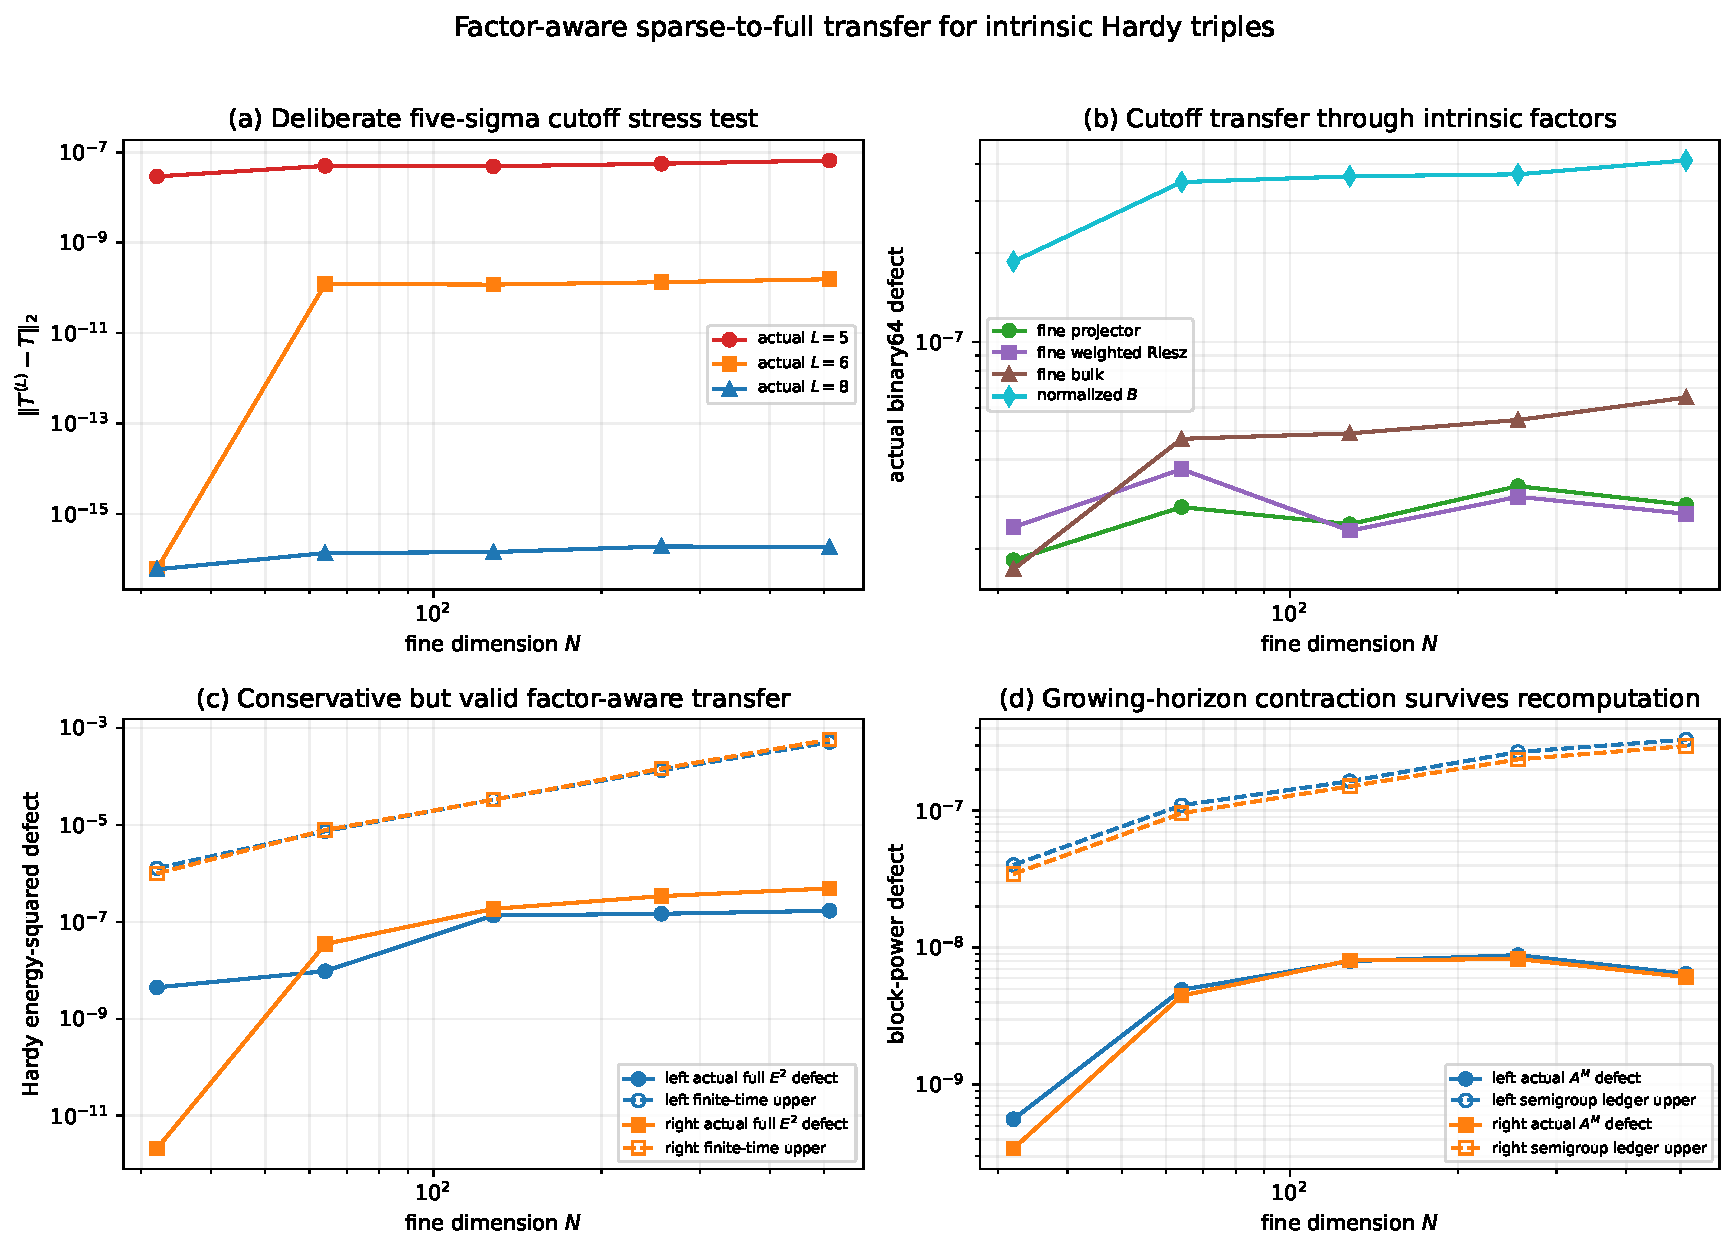
\includegraphics[width=\textwidth]{figures/factor_aware_intrinsic_identification.pdf}
\caption{Factor-aware sparse-to-full audit.  (a) The declared five-sigma
window creates a visible stress defect; six and eight sigma rapidly reach
roundoff.  (b) Recomputed intrinsic factors and the normalized outgoing
coupling.  (c) Actual Hardy-energy changes and conservative finite-time
uppers.  (d) Actual growing-block defects and the semigroup telescoping
ledgers.  All panels are binary64 diagnostics.}
\label{fig:audit}
\end{figure}

\subsection{Outward-rounded arithmetic audit}

A separate 256-bit Arb execution encloses a $3\times2$ coupling, its
perturbation, both normalizations, a factor-aware triple ledger, and six
semigroup powers \citep{Johansson2017,Rump2010}.  It certifies
\[
 \norm{\Delta\widehat B}_{\HS}
 \le1.251468\times10^{-8},
 \qquad
 q_6+d_6\le0.025000445.
\]
This validates outward arithmetic for the formulas.  It is intentionally a
small abstract execution and not an interval eigensolver or production-scale
Riesz enclosure.

\section{Theorem boundary and next gate}

The status after this composition is as follows.

\begin{description}[leftmargin=4.5cm,style=nextline]
 \item[Normalized coupling gate]
 Closed analytically.  The adaptive cutoff becomes even smaller after
 division by the physical coupling scale.

 \item[Factor-aware finite transfer]
 Closed analytically once projector and weighted-Riesz defect uppers are
 supplied.  A common-contour ledger is explicit.

 \item[Growing-horizon robustness]
 Closed analytically.  The certificate uses actual finite semigroup ledgers
 and transports both contraction and the full Hardy upper.

 \item[RH-48--RH-53 synthesis]
 Closed as a conditional theorem with exact exponent budget
 $\alpha_B+\alpha_C\le1/4$.

 \item[Uniform Stage A1 budget]
 Open.  No analytic theorem yet bounds both dyadic Hardy energies uniformly,
 polylogarithmically, or with a proved total power at most $1/4$.

 \item[Uniform intrinsic Riesz modulus]
 Open.  The dense audit observes stability, but the no-go theorem shows that
 an operator cutoff bound alone cannot prove it.

 \item[Unconditional Stage A4]
 Open.  The preceding two premises prevent an unconditional claim despite
 the complete finite-dimensional transfer architecture.
\end{description}

The sharp next target is no longer another fixed-window pilot.  One needs a
dyadically uniform analytic Hardy/Stein trace budget together with either a
strong--weak intrinsic-factor modulus or an outward-rounded contour ledger
on the production family.  If these provide total Hardy exponent at most
$1/4$, \cref{thm:composition} closes the identification theorem immediately.
If every valid budget exceeds $1/4$, the full strict $n\sigma^2\to\infty$
range fails and a stronger mesh schedule must be stated instead.

No result here constructs an arithmetic trace formula, a prime-power
identity, a self-adjoint Hilbert--P\'olya operator, a $T\log T$ counting law,
or a zeta-zero spectral identity, and no Riemann-hypothesis conclusion is
drawn.  The independent TPC twin-prime branch is not a premise of this
theorem.

\section{Reproducibility}

The archive contains theorem code in \path{src/intrinsic_transfer}, the
five-scale pilot, the Arb audit, tests, figure sources, a machine-readable
closure certificate, dependency hashes, and the manuscript.  From this
directory, the main replay is
\begin{verbatim}
PYTHONDONTWRITEBYTECODE=1 /root/math/.venv/bin/pytest -q
OPENBLAS_NUM_THREADS=16 OMP_NUM_THREADS=16 \
  PYTHONDONTWRITEBYTECODE=1 /root/math/.venv/bin/python \
  experiments/run_factor_aware_pilot.py
PYTHONDONTWRITEBYTECODE=1 /root/math/.venv/bin/python \
  experiments/run_arb_transfer_audit.py
PYTHONDONTWRITEBYTECODE=1 /root/math/.venv/bin/python \
  experiments/build_closure_certificate.py
MPLBACKEND=Agg PYTHONDONTWRITEBYTECODE=1 /root/math/.venv/bin/python \
  experiments/make_figures.py
latexmk -pdf -interaction=nonstopmode -halt-on-error main.tex
\end{verbatim}

\section{Conclusion}

The sparse/full gap left by deterministic Hardy tails can be propagated
through recomputed intrinsic factors without choosing eigenvector gauges.
Normalized Haar couplings are stable at twice their relative
Hilbert--Schmidt error, the weighted and unweighted Riesz terms enter through
separate auditable defects, and one growing contracting block survives under
the exact finite semigroup ledger.  These ingredients compose RH-48 through
RH-53 into a single closure theorem with the transparent threshold
$\alpha_B+\alpha_C\le1/4$.

The result also marks the remaining wall precisely.  Nonnormal Riesz
stability is not free, and finite Hardy plateaus do not prove a uniform trace
budget.  Thus the route remains viable and substantially clearer, but its
last analytic premises must still be proved or validated before the
small-noise intrinsic identification can be called unconditional.

\bibliographystyle{plainnat}
\bibliography{references}

\end{document}
